\begin{figure}[htb]
  \begin{center}
    \resizebox{\textwidth}{!}{
      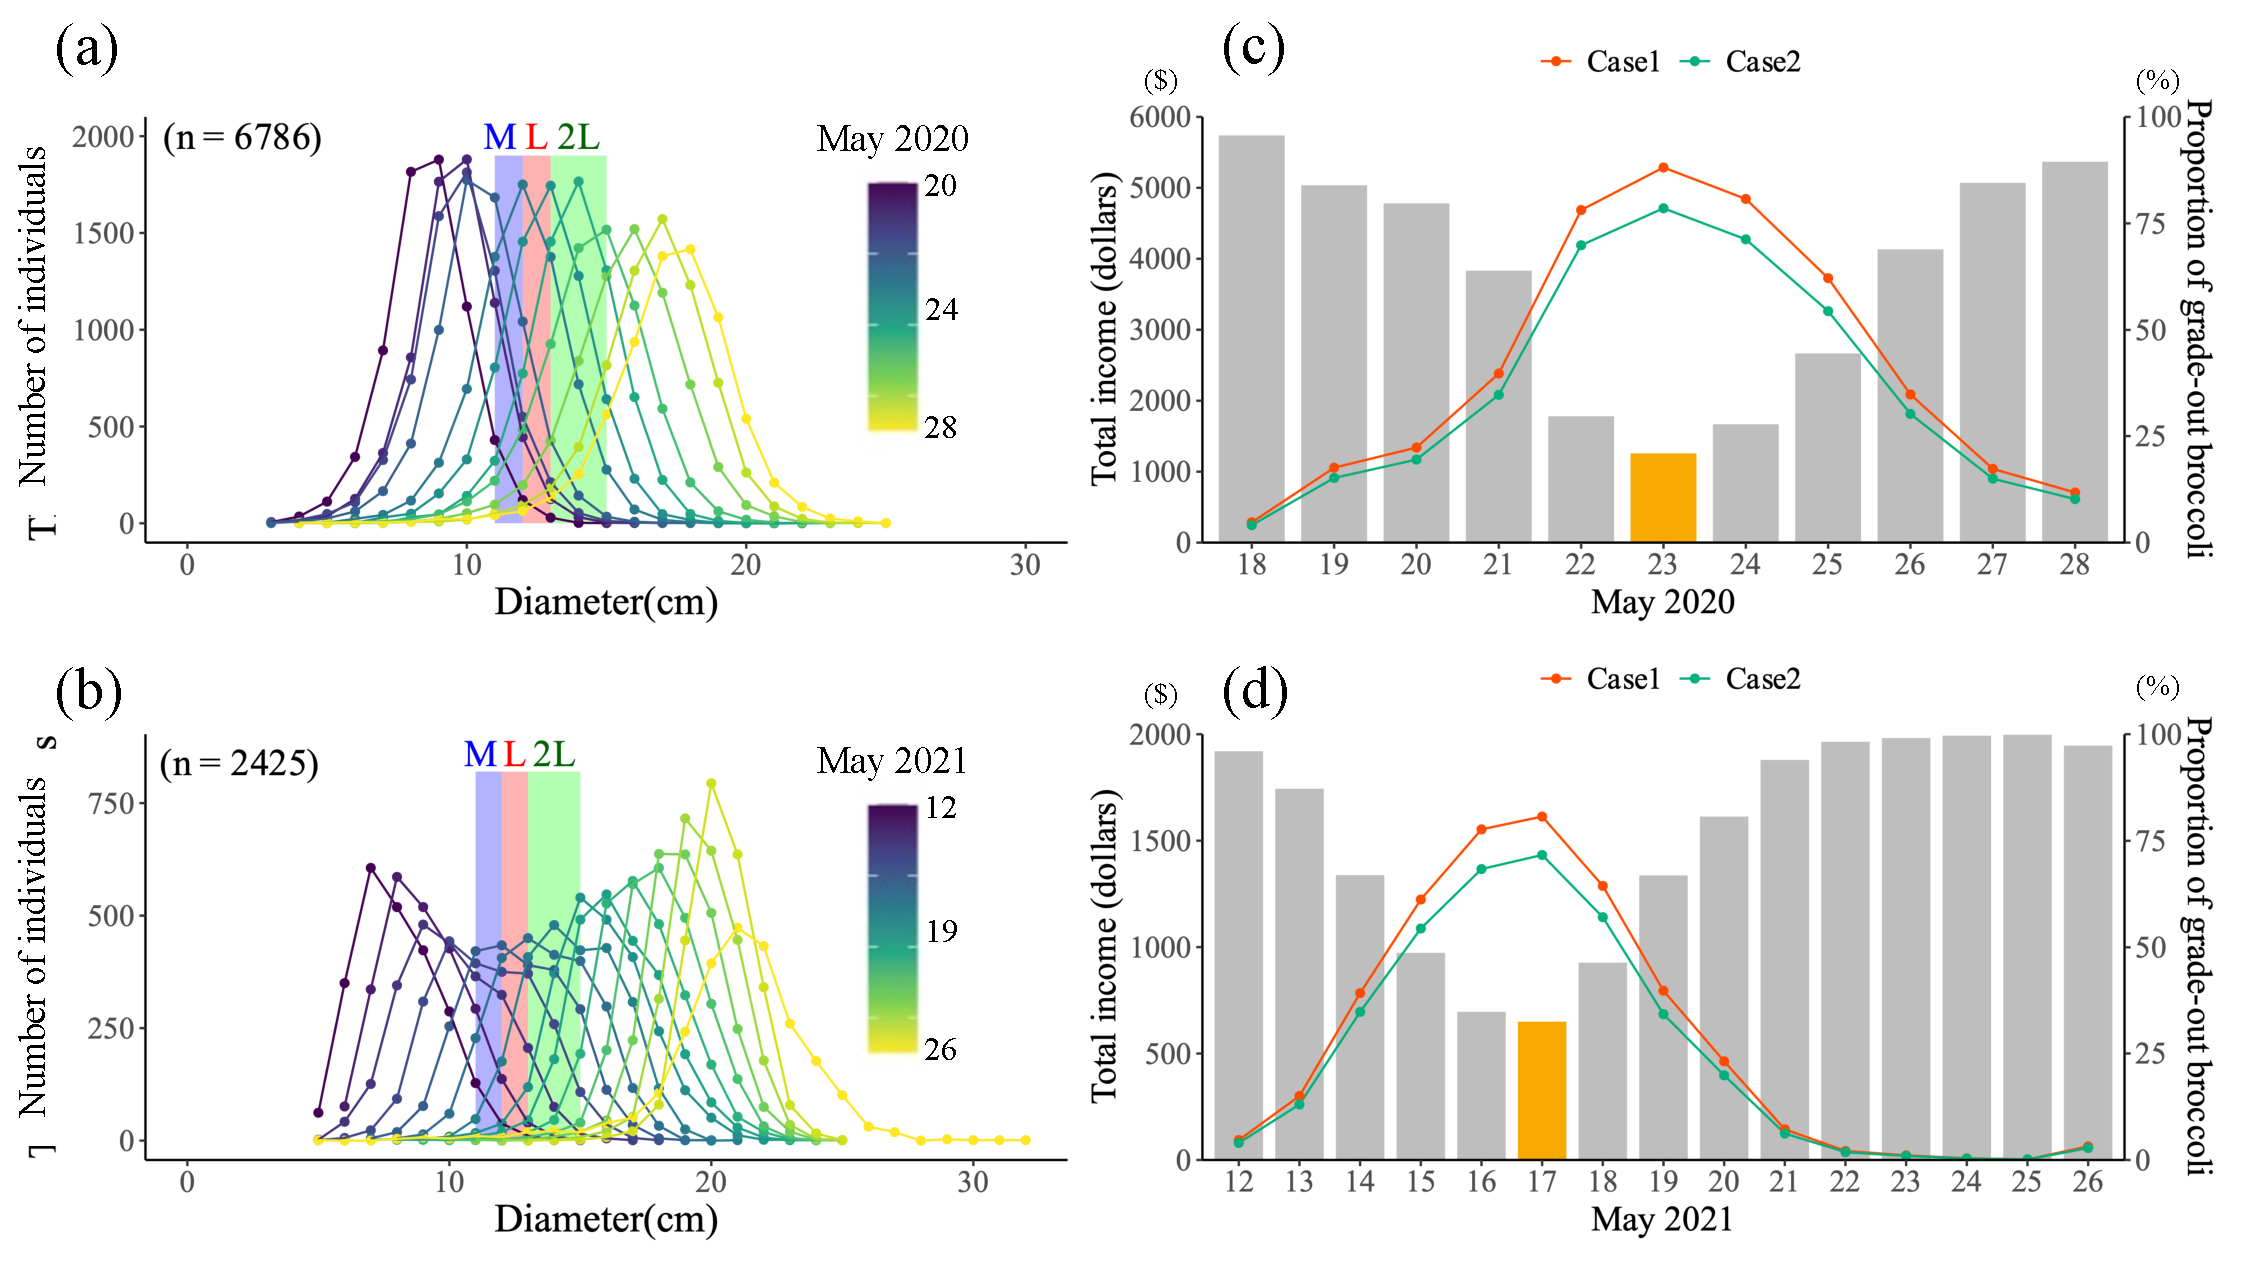
\includegraphics{figures/bro/Fig.3_predict.pdf}
    }
  \end{center}
  \caption[Distribution of predicted head diameter in 2020 and 2021 trials]{
    Distribution of predicted head diameter in (a) 2020 and (b) 2021 trials. 
    The M, L, and 2L sizes meet the shipping standard in the Japanese market 
    (M: 11–12 cm, L: 12–13 cm, and 2L: 13–15 cm). The proportion of non-standard-size broccoli and total income assuming all individuals were harvested for each date in the (c) 2020 and (d) 2021 trials. 
    Yellow pillars indicated the optimal harvest date generating the highest income and lowest wasted broccoli. 
    Case 1 is the largest price difference between each grade (indicates highest profit), and case 2 is the smallest difference (indicates lowest profit).
  }
  \label{fig:bro3}
\end{figure}